\section{전체 구조: Fly-by-Wire}
\label{sec:structure}

\begin{figure*}[t]
\centering
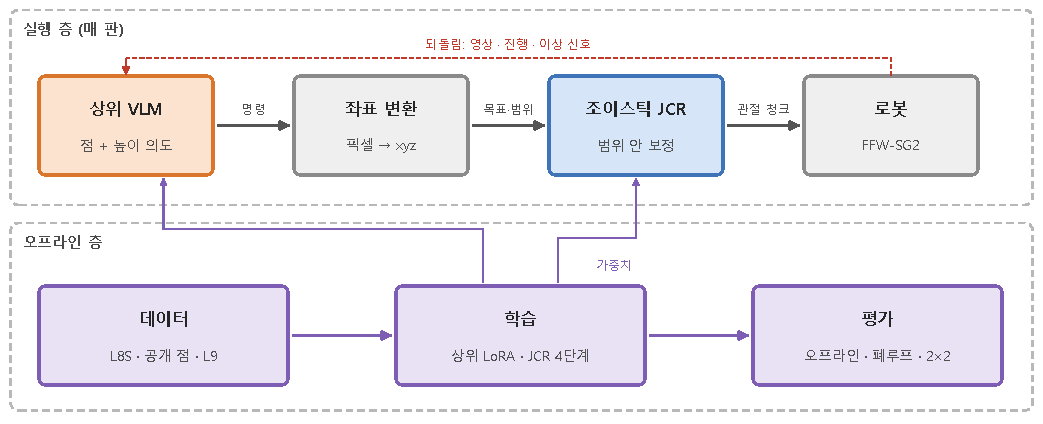
\includegraphics[width=\linewidth]{figures/f1_overview.pdf}
\caption{\textbf{전체 파이프라인.} 위: 실행 층. 상위 VLM이 머리 영상 위의 점과 높이 의도를 내면(재학습 없이 지금 학습한 형식 그대로), 코드 어댑터가 깊이로 xyz를 계산해 대상 마스크·단계·그리퍼 허용·단계별 끌림 세기로 바꿔 조이스틱 JCR에 준다. JCR는 그 끌림을 따라 보정해 로봇에 관절 청크를 보낸다. JCR 보고(접촉·잡기 성공·이상 신호)는 어댑터가 문장으로 바꿔 상위의 `직전 명령과 결과' 입력 칸에 넣는다. 아래: 오프라인 층. 데이터(L8S·공개 점·L9)로 JCR를 학습하고(상위는 동결), 오프라인 점·폐루프·결합 2$\times$2로 평가한다. 세부는 \cref{fig:upper,fig:vla,fig:timeline,fig:train,fig:closs,fig:data}.}
\label{fig:overview}
\end{figure*}

조종사는 조이스틱으로 직접 조종하며 권한을 전부 갖고, 비행 제어 컴퓨터는 조종사가 정한 목적지로 끌어당기며 안정화·보정할 뿐 목적지를 정하지 않고 넓은 안전 범위만 지킨다. Fly-by-Wire에서 조종사는 상위 VLM, 조종간 신호를 비행 제어 컴퓨터가 쓰는 신호로 바꾸는 장치는 코드 어댑터, 비행 제어 컴퓨터는 JCR다(\cref{fig:overview}).

\paragraph{권한.} 명령 권한은 항상 상위에 있다. 목표, 높이 의도, 그리퍼 의도, 진행 평가와 검증은 상위가 낸다. 코드 어댑터(규칙, 학습 없음)가 이를 JCR 명령으로 바꿀 뿐 새 목표를 만들지 않는다. JCR는 어댑터가 정한 끌림을 따라 움직임을 고치고, 이상 신호를 내어 상위를 일찍 다시 부를 근거를 준다. JCR는 과제를 고르거나 상위 목표를 바꾸지 않는다.

\paragraph{한 판의 흐름.} 상위가 목표를 낸다 $\rightarrow$ 어댑터가 명령으로 바꾼다 $\rightarrow$ 실행(1단계는 결정적 실행기, 2단계는 JCR) $\rightarrow$ 도착 뒤 상위에게 다시 묻는다(상위가 학습한 장면 그대로); 상위가 생각하는 1--3\,s 동안 JCR는 정렬·잡기·들기 시작을 이어가 로봇이 멈추지 않는다 $\rightarrow$ 검증 $\rightarrow$ 반복. 잡음·놓음의 확정은 그리퍼 폭·전류를 보는 고유 감각 코드(T1)가 맡고, 상위는 결과를 보고 다음 단계를 고른다.

\paragraph{두 단계로 검증한다.} 1단계는 상위 단독이다. 상위 명령을 결정적 실행기가 평균 약 8\,cm/s의 최소 저크 직선 운동으로 수행하고, 로봇은 상위의 답을 기다린다. 실행기에는 재학습 없는 두 규칙이 있다. 쥐기 전에 깊이로 잰 대상 점을 기억해 두었다가 든 물체가 놓을 곳을 가릴 때 쓰고, `위' 의도가 같은 목표에서 되풀이되면 다음 단계로 넘긴다. 2단계는 실행기 자리에 코드 어댑터 + 조이스틱 JCR를 넣어, 상위가 생각하는 동안 JCR가 이어가며 기다림을 없앤다(\cref{sec:coupling}). 1단계는 결합의 비교 기준으로 남는다.

\paragraph{플랫폼.} 기준 로봇은 ROBOTIS AI Worker FFW-SG2다(7자유도 팔 두 개, 평행 그리퍼, 2자유도 머리, 리프트, 팔마다 100\,Hz 위치 명령). 카메라는 기본 장착분만 쓴다. 머리 ZED Mini 672$\times$376, 손목 RealSense D405 두 대다. 머리는 45$^\circ$가 기본이다. 안전 규칙으로 팔 관절 한 걸음은 0.04\,rad 이하로 묶는다. 시뮬은 Isaac Sim 5.1과 Isaac Lab 2.3이다.
